%!TEX TS-program = xelatex

% Официальный шаблон презентации НИУ ВШЭ в beamer (LaTeX)
% Версия 2.0
% Язык — русский

\documentclass[aspectratio=169]{beamer}

\newbool{russian}
\booltrue{russian}
\usepackage{HSE-theme/beamerthemeHSE}

%%% Работа с русским языком и шрифтами
\usepackage{multirow}
\usepackage{listings} 
\usepackage[dvipsnames]{xcolor}
\usepackage[english,russian]{babel}
\usepackage[no-math]{fontspec}
\usepackage{makecell}
	\IfFontExistsTF{HSE Sans}
		{\newcommand{\presentationfont}{HSE Sans}}
		{\newcommand{\presentationfont}{Arial}}
	\setsansfont{\presentationfont}
	\setmonofont{Courier New}

\usepackage{mathspec}
	\setmathsfont(Digits,Latin,Greek)[Numbers={Lining,Proportional}]{\presentationfont}
	\setmathrm[Numbers={Lining,Proportional}]{\presentationfont}
\uselanguage{russian}
\languagepath{russian}
\deftranslation[to=russian]{Theorem}{Теорема}
\deftranslation[to=russian]{Definition}{Определение}
\deftranslation[to=russian]{Definitions}{Определения}
\deftranslation[to=russian]{Corollary}{Следствие}
\deftranslation[to=russian]{Fact}{Факт}
\deftranslation[to=russian]{Example}{Пример}
\deftranslation[to=russian]{Examples}{Примеры}

\usepackage{booktabs}
\usepackage{array}
\graphicspath{{images/}}


\newcommand{\term}[1]{{\large\textcolor{HSEblue}{#1}}}
\newcommand{\cmd}[1]{\texttt{#1}}
\newcommand{\todo}[1]{\textcolor{red}{[TODO: #1]}}

\newenvironment{demoblock}[1]
	{\begin{exampleblock}{Демо: #1}\small}
	{\end{exampleblock}}

\lstset{ 
    basicstyle=\color{HSEblue}\ttfamily\small,
    numbers=left,
    numberstyle=\color{HSEblue}\ttfamily\scriptsize,
    frame=single,
    rulecolor=\color{HSEblue},
}


%% Информация об авторе и выступлении
\title[Мобильные колесные роботы]{Проектный семинар \\ <<Мобильные колесные роботы>>}
% \subtitle{}
\author[Команда курса]{Дергачев Степан  Алексеевич, \texttt{\href{mailto:sadergachev@hse.ru}{sadergachev@hse.ru}} \\ Муравьев Кирилл Федорович, \texttt{\href{mailto:kmuravev@hse.ru}{kmuravev@hse.ru}}}
\institute{Факультет компьютерных наук НИУ ВШЭ}
\date{10 сентября 2026}

\begin{document}

\frame[plain]{\titlepage}

\begin{frame}
\frametitle{Содержание курса}
\begin{enumerate}
	\item Инструменты разработки: Linux, Docker, ROS~2.
	\item Симуляция мобильного робота: Webots.
	\item Кинематика, одометрия, управление и система координат.
	\item Датчики, оценка состояния и локализация по известной карте.
	\item SLAM и построение карты.
	\item Автономная навигация и алгоритмы планирования: ROS2 Nav2
	\item Практика на реальных роботах.
\end{enumerate}
\end{frame}


\section{Организация курса}

\begin{frame}
\frametitle{Организация курса}

\begin{columns}[T]
\column{0.48\textwidth}
\begin{block}{Теория}
	\begin{itemize}
	\item Знакомство с темой
	\end{itemize}
\end{block}
\column{0.48\textwidth}
\begin{block}{Практика}
	\begin{itemize}
	\item Демонстрации примеров
	\item Выполнение практических работ
	\end{itemize}
\end{block}
\end{columns}
\vfill
\renewcommand{\arraystretch}{1.2} 
\begin{tabular}{>{\centering\arraybackslash}p{0.18\textwidth}>{\raggedright}p{0.74\textwidth}}
\toprule
\term{Модуль} & \term{Содержание} \tabularnewline
\midrule
1 & Основы ROS2, модель робота и оценка состояния
\tabularnewline
2 & Локализация, SLAM, навигация, планирование траекторий
\tabularnewline
3 & Практика на реальных роботах
\tabularnewline
\bottomrule
\end{tabular}
\vfill
\end{frame}




\begin{frame}
\frametitle{Система оценивания}
\[
	O_{\text{итог}} =
	0.25 \cdot O_{\text{экз}} +
	0.15 \cdot O_{\text{пз1}} +
	0.20 \cdot O_{\text{пз2}} +
	0.25 \cdot O_{\text{пз3}} +
	0.15 \cdot O_{\text{акт}}
\]
\vfill
\renewcommand{\arraystretch}{1.2} 
\begin{tabular}{>{\raggedright}p{0.15\textwidth}>{\centering}p{0.20\textwidth}>{\raggedright}p{0.12\textwidth}>{\raggedright}p{0.4\textwidth}}
\toprule
\term{Компонент} & \term{Обозначение} &\term{Вес} & \term{Содержание} \tabularnewline
\midrule
Экзамен-защита & $O_{\text{экз}}$ & 25\% & \small Индивидуальная защита результатов после выполнения практических заданий. \tabularnewline
\multirow{3}{0.1\textwidth}{Практические задания} & $O_{\text{пз1}}$ & 15\% &  \multirow{3}{0.4\textwidth}{Решение практических заданий по темам курса}\tabularnewline
 & $O_{\text{пз2}}$ & 20\% &  \tabularnewline
 & $O_{\text{пз3}}$ & 25\% &  \tabularnewline
Активность & $O_{\text{акт}}$ & 15\% & Активность в выполнении практических заданий на парах, прогресс в выполнении \tabularnewline
\bottomrule
\end{tabular}
\end{frame}

\begin{frame}
\frametitle{Выполнение практических работ и активность}
	\begin{block}{Формат}
		\begin{itemize}
			\item 1-2 модули -- индивидуальное выполнение
			\item 3 модуль -- возможно групповое выполнение
		\end{itemize}
	\end{block}
	\begin{block}{Мягкие дедлайны}
		\begin{itemize}
			\item сдача до дедлайна: 100\% оценки
			\item опоздание до 7 дней после: 75\% оценки
			\item опоздание до 14 дней после: 50\% оценки
		\end{itemize}
	\end{block}
\vfill
\end{frame}

\begin{frame}
\frametitle{Выполнение практических работ и активность}
\begin{block}{Оценивание практики. Что нужно сдать:}
\begin{itemize}
	\item Репозиторий на GitHub: код, конфиги, пояснения для воспроизведения результата (README).
	\item Демонстрационное видео: короткая запись экрана с запуском и наблюдаемым результатом.
\end{itemize}
\end{block}
\begin{block}{Оценивание активности}
	\begin{itemize}
	\item Оценивается по наблюдаемому прогрессу на паре.
	\item Присутствие необходимо, но не достаточно.
	\item Содержательные вопросы тоже считаются активностью.
\end{itemize}
\end{block}
\end{frame}

\begin{frame}
\frametitle{Автомат и экзамен}
\begin{block}{Условия автомата}
\[
	O_{\text{акт}} \ge 7.5
	\quad \text{и} \quad
	\frac{0.15 \cdot O_{\text{пз1}} + 0.20 \cdot  O_{\text{пз2}} + 0.25 \cdot  O_{\text{пз3}}}{0.60} \ge 7.5
\]
\end{block}
\begin{block}{Экзамен-защита}
\begin{itemize}
	\item Если автомат есть, сдавать экзамен не требуется.
	\item На экзамене нужно показать результаты практических работ и ответить на вопросы по выполнению.
	\item Если практическое задание не выполнено, могут быть вопросы по предполагаемому пути выполнения или вопросы по эталонному решению
\end{itemize}
\end{block}
\end{frame}

\section{Инструменты разработки}

\begin{frame}[fragile]
\frametitle{Командная строка Linux}
\begin{block}{Общий вид команды}
\begin{center}
	\cmd{[VARIABLE=value] command  [flags]  [arguments]}.
\end{center}
\begin{itemize}
	\item \texttt{VARIABLE=value} -- переменная среды
	\item \texttt{command} -- название утилиты/программы/команды
	\item \texttt{flags} -- флаги/опции запуска
	\item \texttt{arguments} -- аргументы запуска (могут быть обязательными или необязательными, относиться к флагам и нет)
\end{itemize}
\end{block}
\begin{block}{Работа с командной строкой}
\begin{itemize}
	\item Команды работают относительно текущей директории.
	\item Автодополнение (\cmd{Tab}), история команд (стрелки, \cmd{Ctrl+R}) и сочетания клавиш (\cmd{Ctrl+A}, \cmd{Ctrl+E}, \cmd{Ctrl+L} и т.д.) экономят время
\end{itemize}
\end{block}
\vfill
\end{frame}



\begin{frame}[fragile]
\frametitle{Командная строка Linux}
\begin{block}{Стандартные потоки ввода-вывода}
\begin{itemize}
	\small
	\item \texttt{stdin} — входные данные (дескриптор: 0)
	\item \texttt{stdout} — обычный вывод (дескриптор: 1)
	\item \texttt{stderr} — сообщения об ошибках (дескриптор: 2)
\end{itemize}
\end{block}
\begin{block}{Перенаправление ввода и вывода}
\begin{itemize}
	\small
	\item \cmd{command > result.txt} -- записать stdout в файл
	\item \cmd{command >> result.txt} -- дописать stdout в конец файла
	\item \cmd{command 2> errors.txt} -- записать stderr в файл
	\item \cmd{command > all.txt 2>\&1} -- записать stdout и stderr
	\item \cmd{command < input.txt} -- прочитать stdin из файла
	\item \cmd{command1 | command2} -- передать stdout следующей команде
	\item \cmd{command | tee result.txt} -- вывести на экран и записать в файл
	\item \cmd{command > /dev/null} -- отбросить вывод
\end{itemize}
\end{block}
\vfill
\end{frame}




\begin{frame}[fragile]
\frametitle{Командная строка Linux}
\begin{columns}[T]
\column{0.45\textwidth}
\begin{block}{Навигация и файлы}
	\begin{itemize}
	\item \cmd{pwd}, \cmd{cd}, \cmd{ls},  \cmd{tree}
	\item \cmd{mkdir}, \cmd{touch}, \cmd{cp}, \cmd{mv}, \cmd{rm}
	\item \cmd{cat}, \cmd{less}, \cmd{head}, \cmd{tail}, \cmd{nano}
	\item \cmd{which}, \cmd{find} 
\end{itemize}
\end{block}
\column{0.50\textwidth}
\begin{block}{ОС, процессы и диагностика}
	\begin{itemize}
	\item \cmd{ps}, \cmd{htop}, \cmd{pgrep}, \cmd{kill}, \cmd{pkill}, 
	\item \cmd{grep}, 
	\item \cmd{chmod}, \cmd{sudo}, \cmd{whoami}, \cmd{id}
	\item \cmd{echo \$VARIABLE}, \cmd{env}, \cmd{export VARIABLE=10}
\end{itemize}
\end{block}

\end{columns}
\vfill
\end{frame}

\begin{frame}[fragile]
\frametitle{SSH и удалённая разработка}
\begin{itemize}
	\item \term{SSH (Secure Shell)} -- сетевой протокол, который позволяет управлять компьютерами удаленно через командную строку.
	\item Зачастую необходим в робототехнике при подключении к бортовому компьютеру робота
	\item VS Code (с набором расширений Remote Development) позволяет открыть удалённую папку почти как локальный проект.
\end{itemize}
\vfill
\begin{block}{Примеры:}
\begin{itemize}
\item \cmd{ssh user@host\_address} -- подключение к удаленному компьютеру\\
\item \cmd{scp /local-path/file user@host\_address:/remote-path/} -- загрузить файл на удаленный компьютер\\
\item \cmd{scp user@host\_address:/remote-path/file /local-path/} -- скачать файл с удаленного компьютера
\end{itemize}

\end{block}
\end{frame}

\section{Docker}

\begin{frame}
\frametitle{Docker}
\term{Docker} позволяет запускать приложения в изолированном и воспроизводимом окружении.
\vfill
\begin{columns}[T]
\column{0.48\textwidth}
\begin{block}{Образ}
	\begin{itemize}
	\item Шаблон окружения.
	\item Собирается из \cmd{Dockerfile}
	\item Содержит образ ОС, установленные пакеты и загруженные файлы.
\end{itemize}
\end{block}
\column{0.48\textwidth}
\begin{block}{Контейнер}
\begin{itemize}
	\item Запущенный экземпляр образа
	\item Включает запущенные процессы, изолированные от основной среды
	\item Может использовать сеть и примонтированные тома (volumes) хост-системы
\end{itemize}
\end{block}
\end{columns}
\end{frame}

\begin{frame}[fragile]
\frametitle{Docker Compose}
\vfill
\term{Docker Compose} позволяет управлять и запускать контейнеры  (или группу контейнеров) с помощью одного конфигурационного YAML-файла
\vfill
\begin{center}
	\begin{minipage}{0.7\textwidth}
\begin{lstlisting}
services:
    ros2-base:
        build:
            context: .
            dockerfile: docker/Dockerfile
        image: mobile-robots:jazzy
        volumes:
            - ./src:/home/devuser/robot_ws/src
        environment:
            DISPLAY: ${DISPLAY}
\end{lstlisting}
  \end{minipage}
\end{center}
\end{frame}


\begin{frame}
\frametitle{Docker:  Примеры команд}
\vfill
\begin{columns}[T]
\column{0.48\textwidth}
\term{Docker}
\begin{itemize}
	\item  \cmd{docker images}
	\item  \cmd{docker pull}
	\item  \cmd{docker build}
	\item  \cmd{docker run}
	\item  \cmd{docker ps}
	\item  \cmd{docker exec}
	\item  \cmd{docker start}
	\item  \cmd{docker stop}
	\item  \cmd{docker rm}
\end{itemize}
\column{0.48\textwidth}
\term{Docker Compose}
\begin{itemize}
	\item \cmd{docker compose build}
	\item \cmd{docker compose up}
	\item \cmd{docker compose ps}
	\item \cmd{docker compose exec}
	\item \cmd{docker compose stop}
	\item \cmd{docker compose down}
\end{itemize}
\end{columns}
\end{frame}


\begin{frame}
\frametitle{Зачем нам Docker и Docker Compose}
\begin{block}{Docker обеспечивает:}
	\begin{itemize}
	\item Всегда фиксированные версии библиотек и пакетов
	\item Изоляцию зависимостей от основной системы
	\item Хранение конфигурации рядом с исходным кодом в Git
	\item Воспроизводимую сборку рабочего окружения
\end{itemize}
	
\end{block}
\end{frame}


\begin{frame}
\frametitle{VS Code: Полезные расширения}
\begin{itemize}
	\item Remote Development Pack, Docker Extension Pack, Docker DX -- удаленная разработка
	\item Python, Pylance, Python Environments, Python Debugger, Black Formatter, Jupyter Extension -- разработка на Python
	\item С/C++ Extension Pack, clangd, Clang-Format -- разработка на C++
	\item Markdown, XML, YAML, Edit CSV и др. -- поддержка языков разметки и различных типов файлов.
\end{itemize}
\vfill
\end{frame}

\section{ROS}

\begin{frame}
\frametitle{Robot Operating System}
\begin{block}{}
\term{Robot Operating System (ROS)} -- это набор библиотек, инструментов и соглашений для сборки робототехнических систем из взаимодействующих процессов.
\end{block}

\begin{columns}
	\column{0.68\textwidth}
	\begin{itemize}
		\item Разделение системы на независимые компоненты: драйверы, обработка данных с датчиков, SLAM, планирование, управление.
		\item Соглашение о форматах сообщений и интерфейсах между компонентами.
		\item Механизмы запуска, наблюдения, записи и воспроизведения поведения системы.
		\item Доступность готовых пакетов.
	\end{itemize}
	\column{0.3\textwidth}
	
\includegraphics[width=0.9\columnwidth]{ros_jazzy.png}
\end{columns}


\end{frame}

% \begin{frame}
% \frametitle{Зачем нужен ROS~2}
% \begin{itemize}

% \end{itemize}
% \vfill
% \begin{exampleblock}{Пример}
% Один процесс публикует данные LiDAR, второй строит карту, третий планирует путь, четвёртый отправляет команды на колёса.
% \end{exampleblock}
% \end{frame}

\begin{frame}
\frametitle{ROS~1 и ROS~2}
\centering
\renewcommand{\arraystretch}{1.2} 
\begin{tabular}{>{\raggedright}p{0.24\textwidth}>{\raggedright}p{0.3\textwidth}>{\raggedright}p{0.3\textwidth}}
\toprule
 & \multicolumn{1}{c}{\term{ROS~1}} & \multicolumn{1}{c}{\term{ROS~2}}\tabularnewline
\midrule
Связь процессов & Централизованная, требуется запуск \texttt{roscore} & Децентрализованная
\tabularnewline

Реальное время & Ограниченная поддержка & Потенциал есть, нужна настройка
\tabularnewline

Сеть & Собственный стек на основе TCP/UDP. Проще настраивается. & Протокол DDS, большая вариативность, но сложная настройка
\tabularnewline
\midrule
Состояние & \textcolor{HSEred}{Больше не поддерживается} & \textcolor{HSEgreen}{Активно развивается}
\tabularnewline
\bottomrule
\end{tabular}
\end{frame}


\begin{frame}
\frametitle{Система версий ROS и Ubuntu}
% \begin{itemize}
% 	\item ROS~2 распространяется по дистрибутивам: Humble, Iron, Jazzy, Kilted и т.д.
% 	\item Каждый дистрибутив ROS~2 обычно привязан к конкретным версиям Ubuntu.

% 	\item В репозитории курса используется ROS~2 Jazzy на базе Ubuntu 24.04 Noble.
% \end{itemize}

\begin{columns}
	\column{0.49\textwidth}
	\begin{itemize}
		\item ROS~2 распространяется дистрибутивами: Humble, Iron, Jazzy, Kilted и т.д.
		\item Дистрибутивы выходят раз в год, каждые два года -- LTS релиз
		\item Версия ROS привязана к LTS версиям Ubuntu
	\end{itemize}
	\column{0.49\textwidth}
	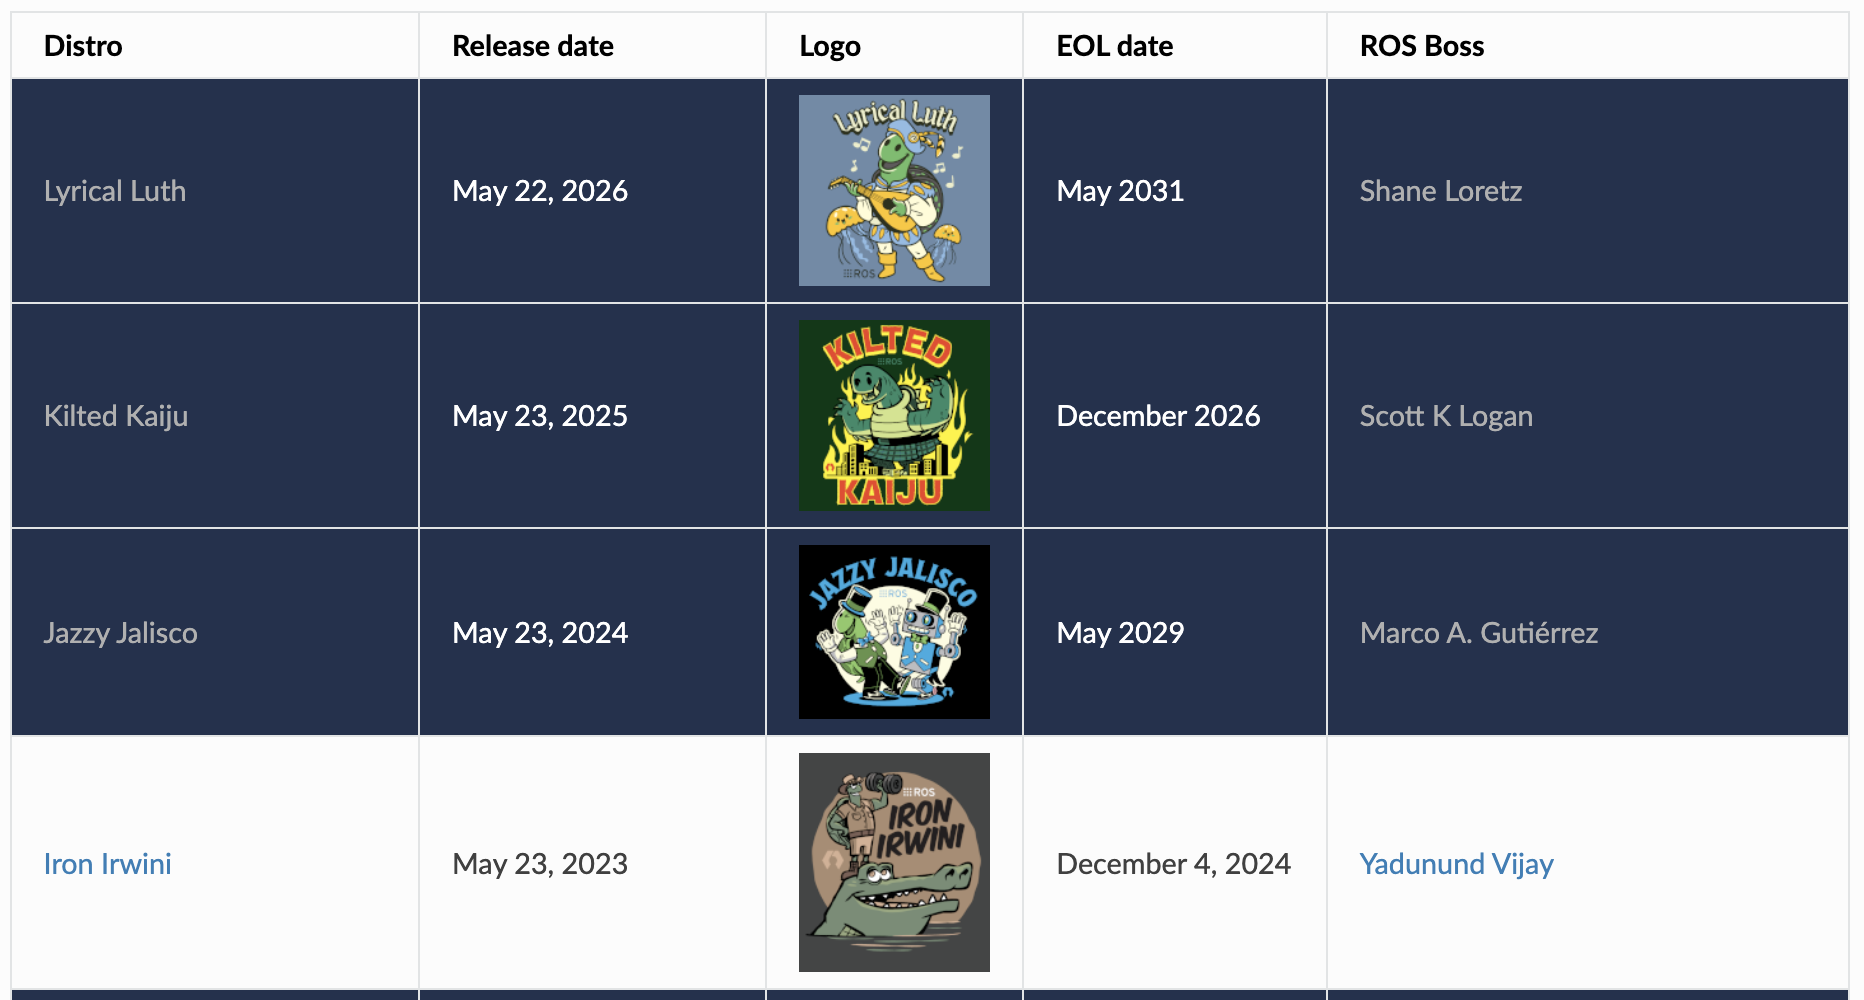
\includegraphics[width=0.8\columnwidth]{ros_versions.png}%
	\vspace{5 pt}\\
	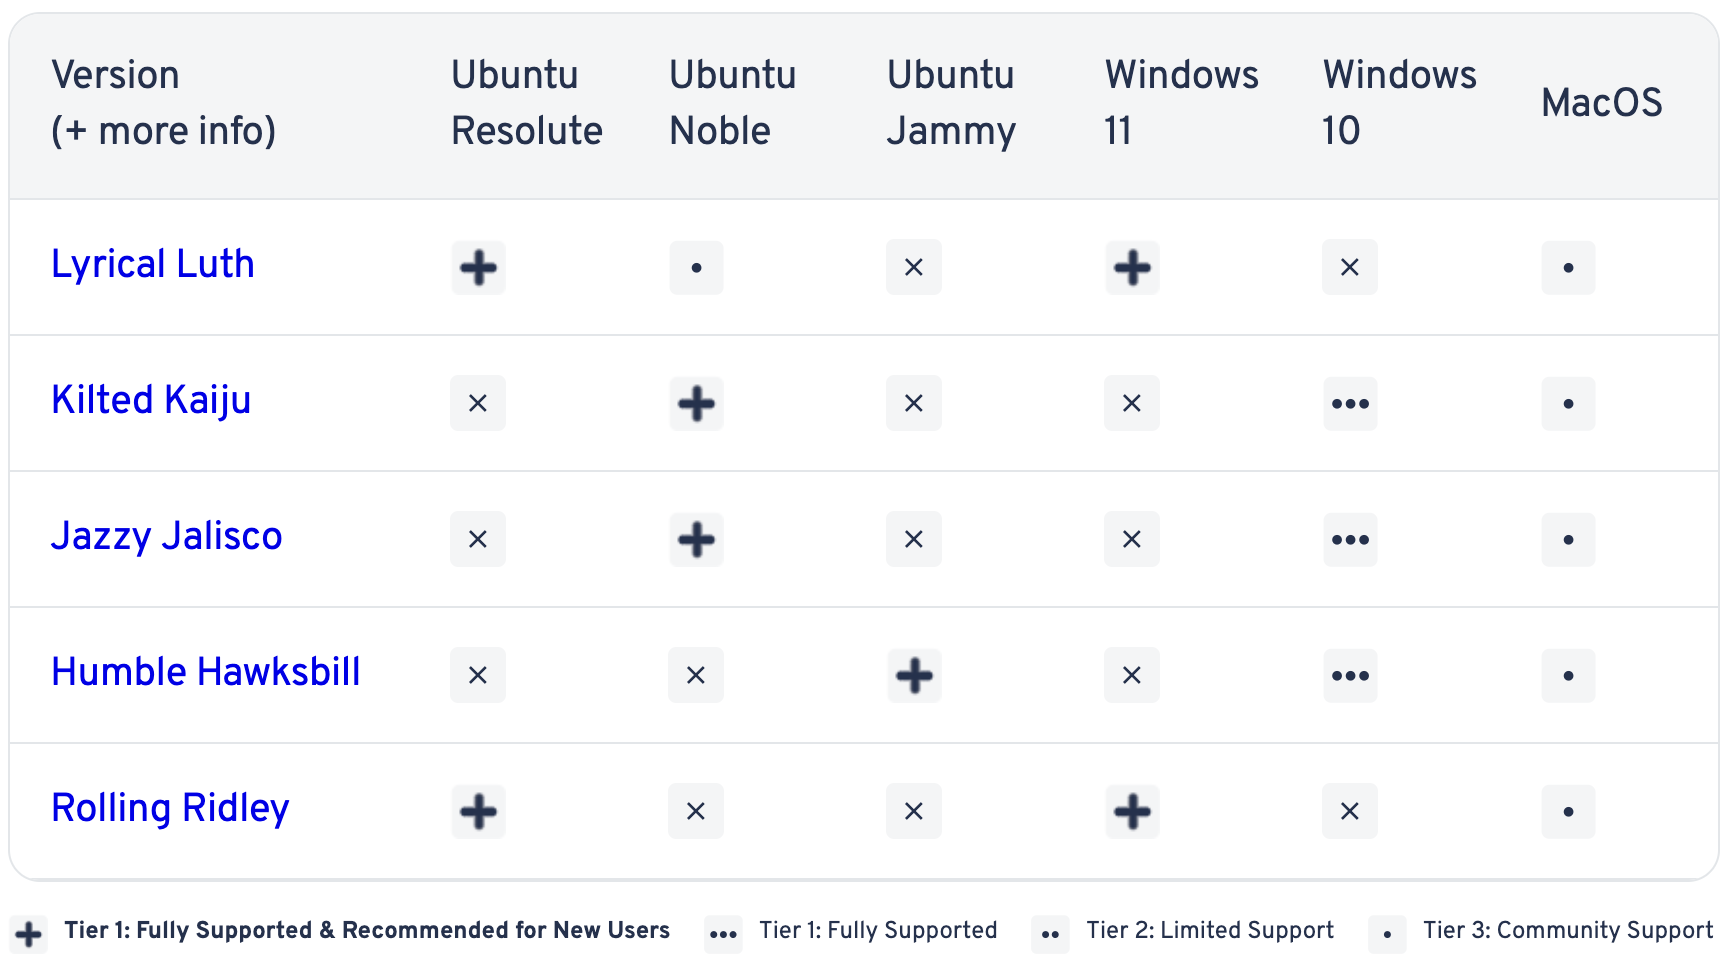
\includegraphics[width=0.8\columnwidth]{ros_ubuntu_versions.png}

\end{columns}

\vfill
% \begin{alertblock}{Практическое следствие}
% Команда из интернета может не работать, если она написана для другой версии ROS~2 или Ubuntu.
% \end{alertblock}
\end{frame}



\begin{frame}
\frametitle{ROS~2: Основные концепции}
\begin{itemize}
	\item \term{Node (узел)} -- процесс или компонент, который выполняет какую-либо задачу.
	\item \term{Topic} -- механизм передачи сообщений между узлами через именованный канал.
	\item \term{Service} -- механизм передачи запроса и ответа между узлами для выполнения коротких операций.
	\item \term{Action} -- механизм передачи запроса и ответов о ходе выполнения долгих задач с обратной связью.
	\item \term{Parameters} -- механизм настройки узлов во время запуска или выполнения.
	\item \term{Launch-файлы} -- конфигурационные/скриптовые файлы с описанием того, что и как запустить вместе.
\end{itemize}
\end{frame}

\begin{frame}
\frametitle{ROS2 Topic}
\begin{columns}
	\column{0.65\textwidth}
	\begin{itemize}
		\item Publisher публикует сообщения, не ожидая ответа.
		\item Subscriber получает сообщения через функцию-callback.
		\item Один topic может иметь несколько publishers и subscribers.
		\item Все участники должны использовать совместимый тип сообщения.
	\end{itemize}
	\column{0.29\textwidth}
	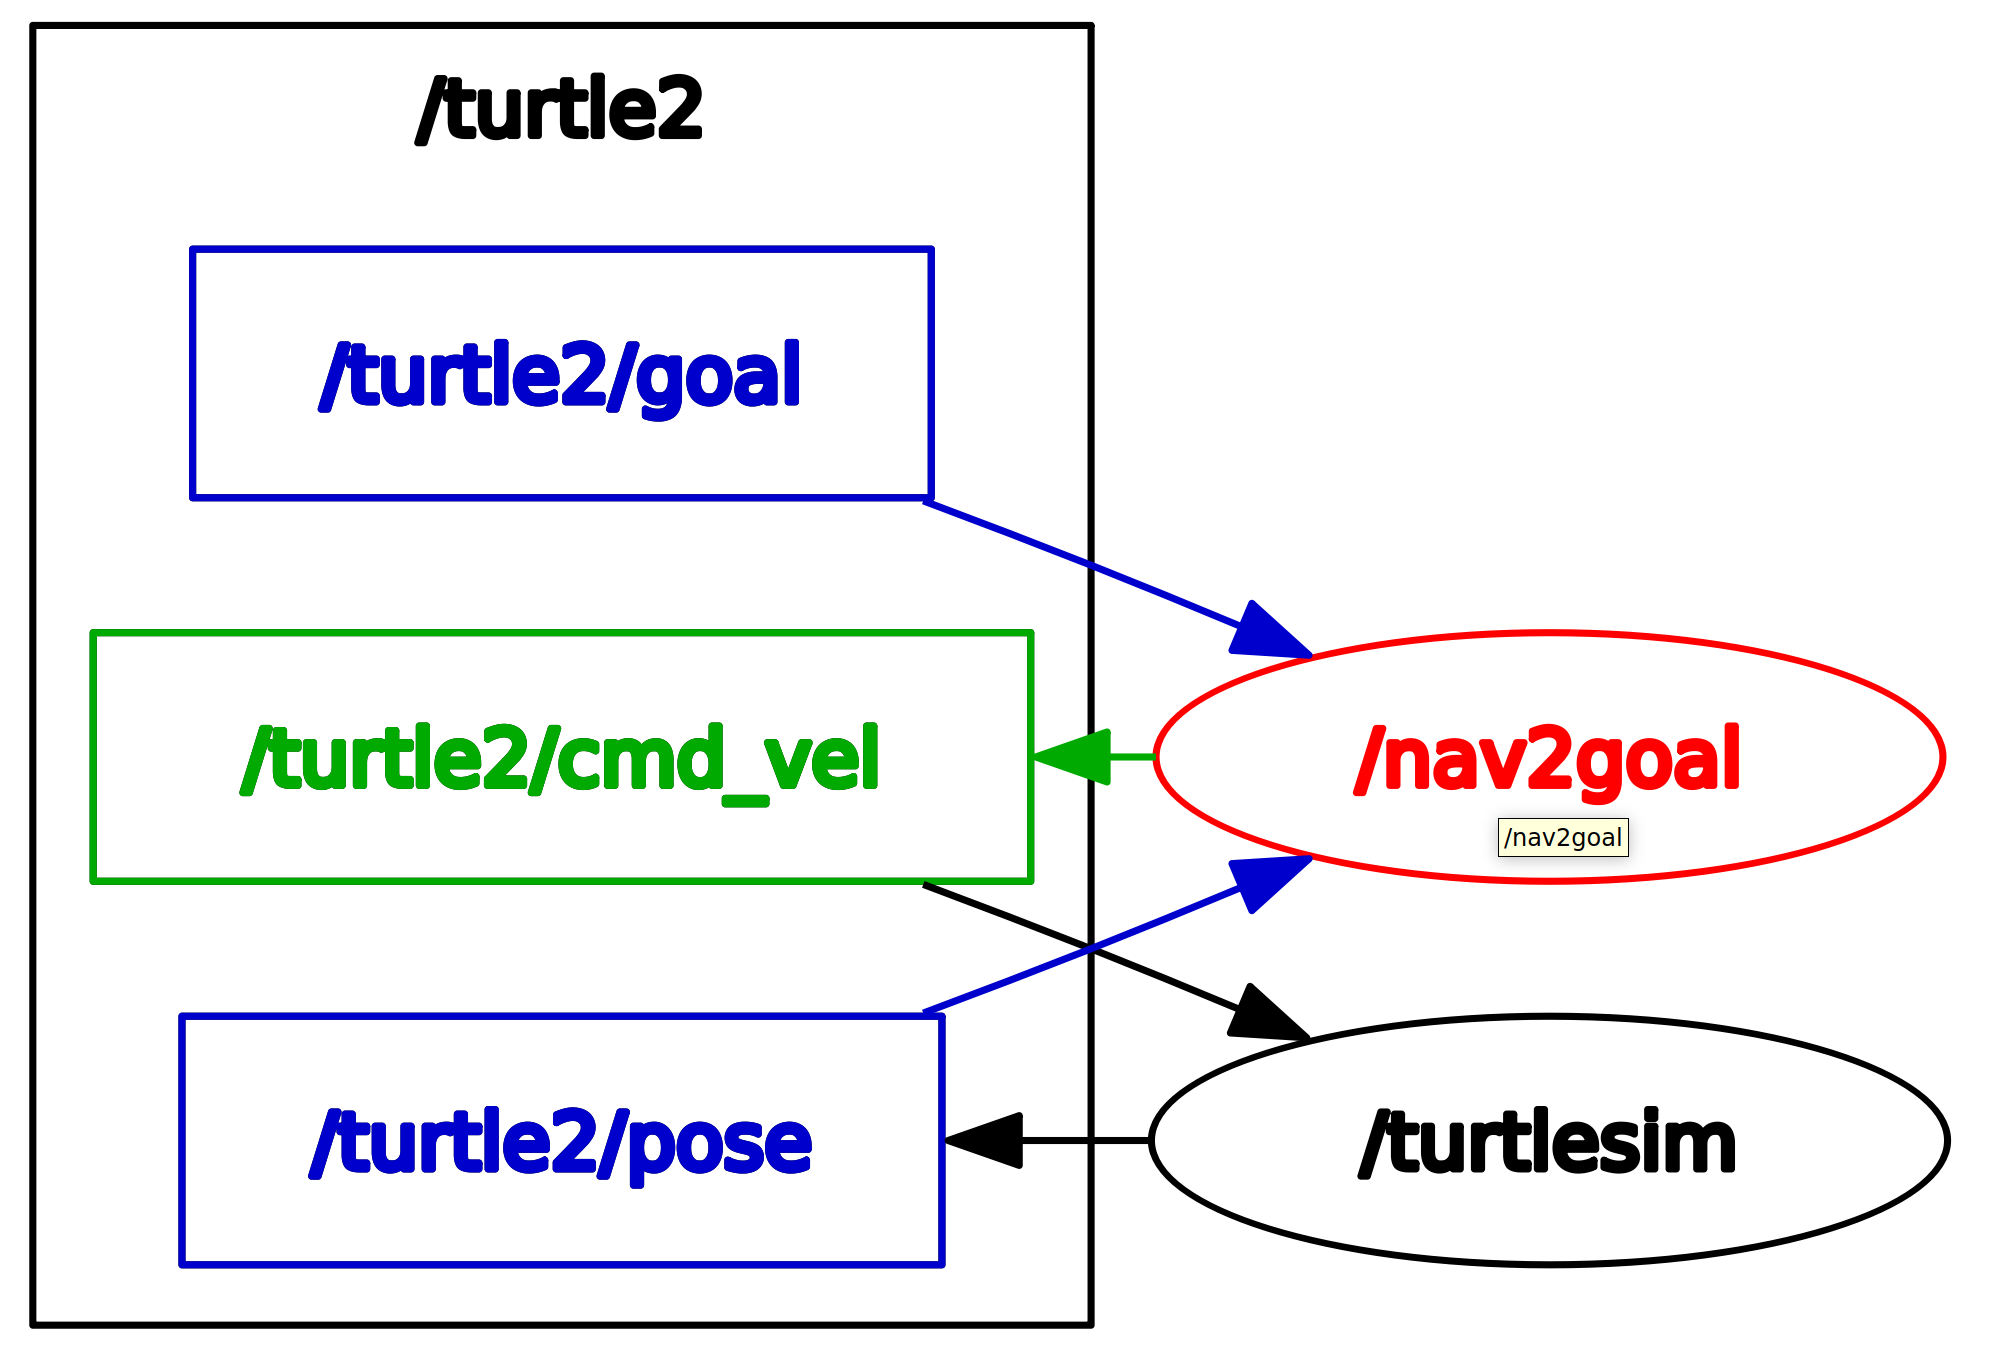
\includegraphics[width=1.0\columnwidth]{topics.png}%
\end{columns}

\end{frame}

\begin{frame}
\frametitle{ROS2 Topic}
\begin{columns}
	\column{0.65\textwidth}
	\begin{block}{Примеры топиков и типов сообщений:}
		\footnotesize
		\cmd{/turtle1/cmd\_vel} -> \cmd{geometry\_msgs/msg/Twist} \\
		\cmd{/turtle1/pose} -> \cmd{turtlesim/msg/Pose}
	\end{block}
	\begin{block}{Примеры диагностики:}
		\footnotesize
		\cmd{ros2 topic list}\\
		\cmd{ros2 topic type /turtle1/pose}\\
		\cmd{ros2 topic info /turtle1/pose}\\
		\cmd{ros2 topic echo /turtle1/pose}\\
		\cmd{ros2 topic hz /turtle1/pose}\\
		\cmd{ros2 interface show geometry\_msgs/msg/Twist}
	\end{block}
	\column{0.29\textwidth}
	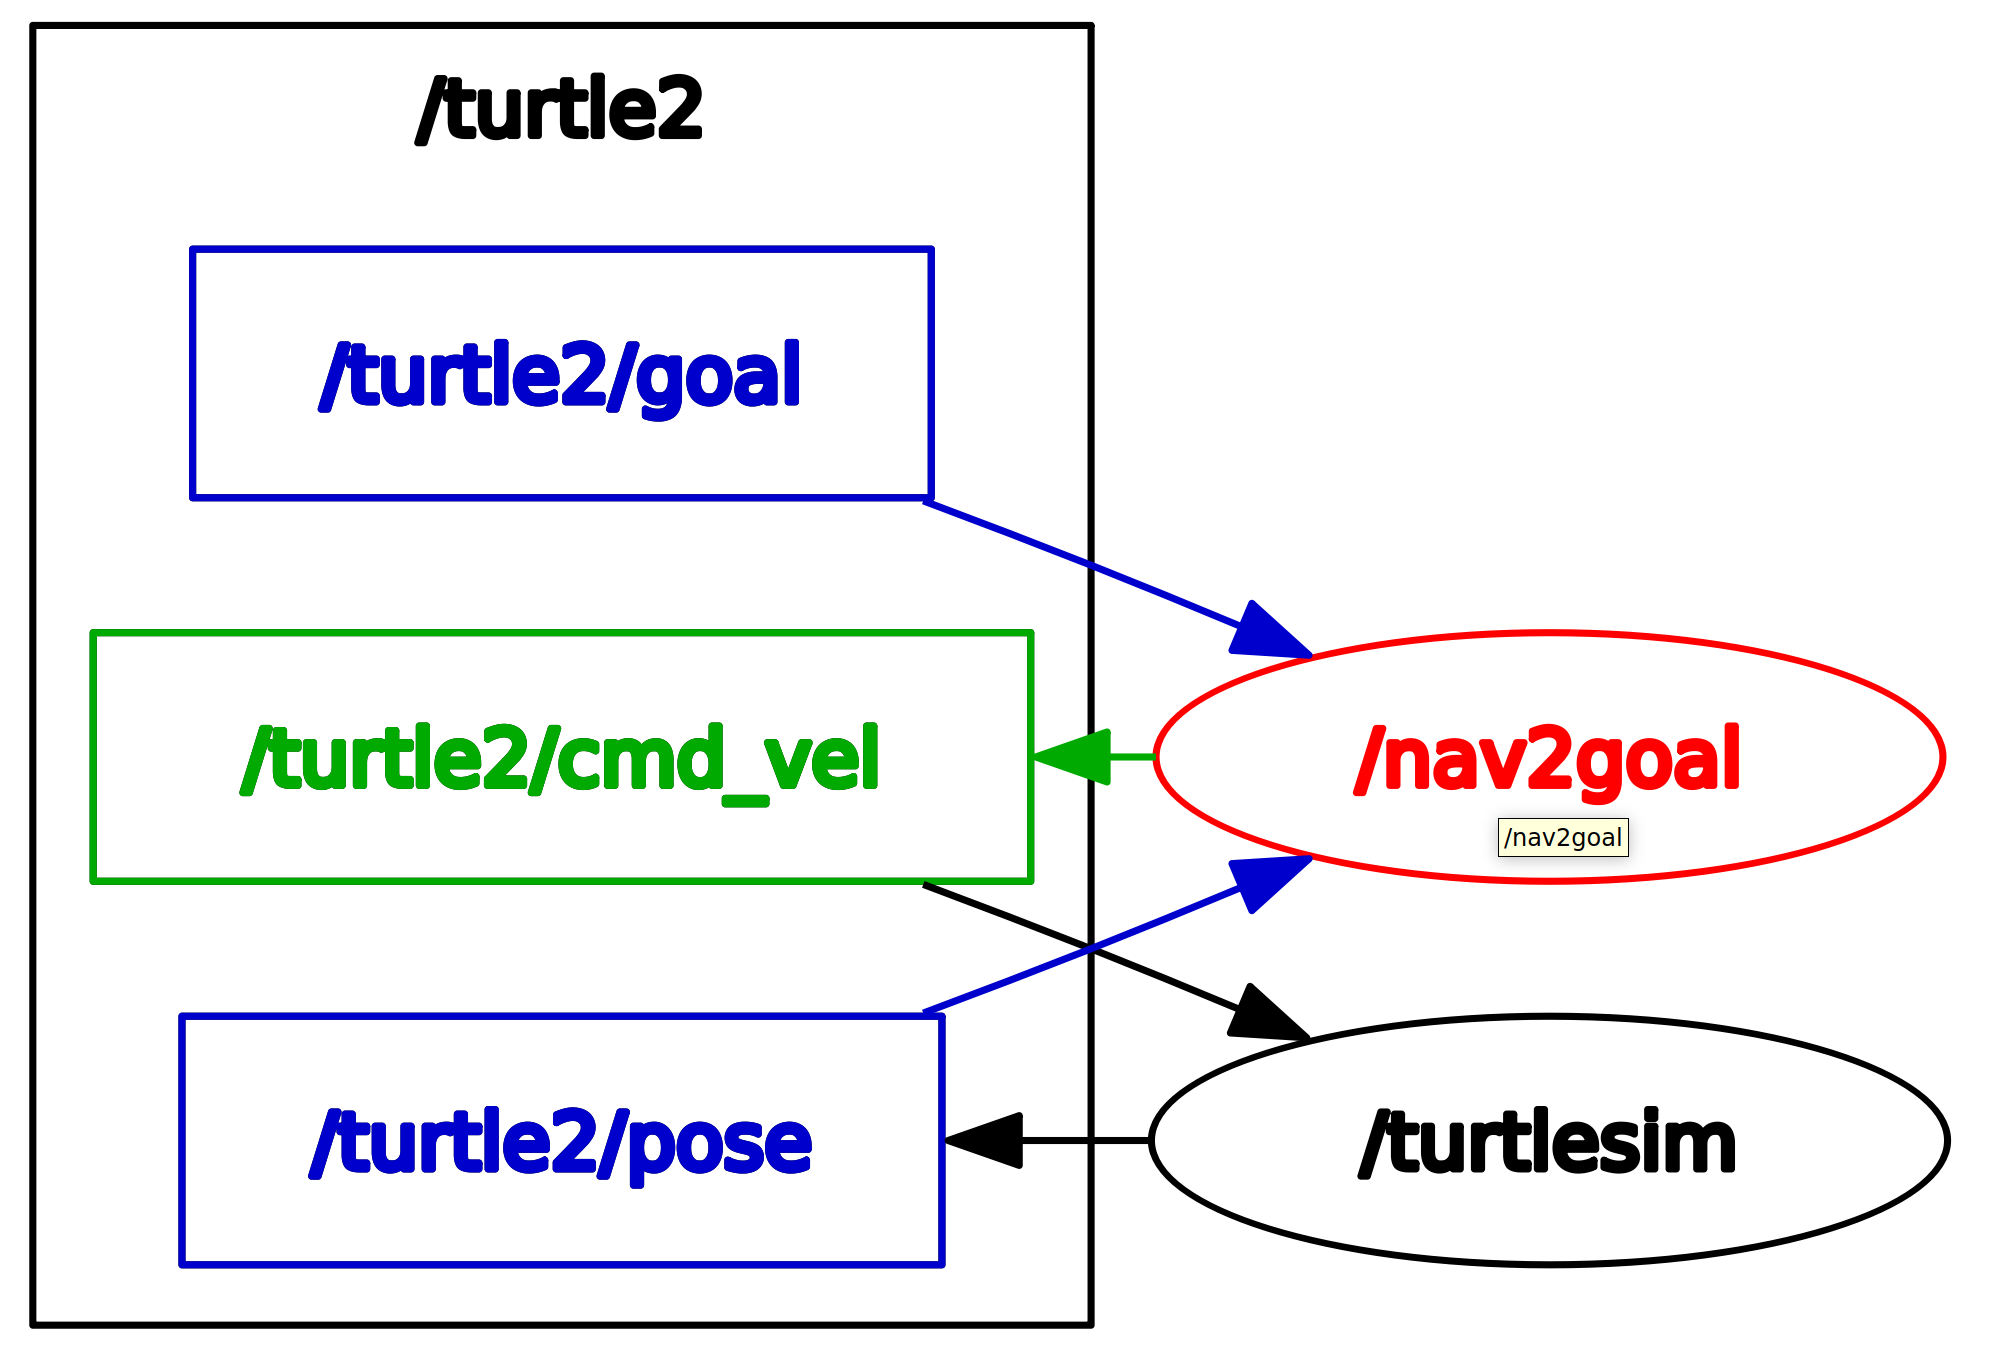
\includegraphics[width=1.0\columnwidth]{topics.png}%
\end{columns}

\begin{block}{Публикация:}
\footnotesize
\cmd{ros2 topic pub /turtle1/cmd\_vel geometry\_msgs/msg/Twist \textbackslash \\
'linear: x: 0.0 y: 0.0 z: 0.0 angular: x: 0.0 y: 0.0 z: 0.0'}
\end{block}

\end{frame}

\begin{frame}
\frametitle{ROS2 service и action}
\begin{columns}[T]
\column{0.48\textwidth}
\begin{block}{Service}
\small
\begin{itemize}
	\item Клиент отправляет запрос, сервер выполняет короткую операцию и возвращает ответ
\end{itemize}
\end{block}
\column{0.48\textwidth}
\begin{block}{Action}
\small
\begin{itemize}
\item Клиент отправляет цель и может получать информацию о ходе выполнения.
\end{itemize}
\end{block}
\end{columns}
\vfill
\begin{block}{Примеры:}
\small
\cmd{ros2 service list} \\
\cmd{ros2 service type /spawn} \\
\cmd{ros2 service info /spawn} \\
\vspace{5pt}
\cmd{ros2 action list}\\
\cmd{ros2 action type /turtle1/rotate\_absolute}\\
\cmd{ros2 action info /turtle1/rotate\_absolute}
\end{block}
\end{frame}

\begin{frame}
\frametitle{Инструменты ROS~2 для диагностики}
\begin{itemize}
	\item CLI интерфейс: \cmd{ros2 node ...}, \cmd{ros2 topic ...}, \cmd{ros2 service ...}, \cmd{ros2 action ...}
	\item Граф связей между узлами: \cmd{rqt\_graph}
	\item Запись и воспроизведение данных: \cmd{ros2 bag}
	\item Инструменты визуализации \cmd{rviz} и \cmd{Foxglove}
	\item Логи узлов в топиках \cmd{/rosout} и \cmd{/diagnostics}
\end{itemize}

\end{frame}

\begin{frame}
\frametitle{ROS~2 Workspace и ROS2 пакеты}
\begin{itemize}
\item Пакет является минимальной единицей организации кода в ROS.
\item ROS~2 Workspace -- рабочая директория, где хранятся ваши пакеты
\item Установка зависимостей утилитой \texttt{rosdep}, сборка пакетов утилитой \texttt{colcon}:
\begin{center}
	\cmd{colcon build --symlink-install}
\end{center}
\item Структура workspace:
\begin{itemize}
	\item \cmd{src/}: исходный код пакетов.
	\item \cmd{build/}: промежуточные файлы сборки.
	\item \cmd{install/}: результат сборки.
	\item \cmd{log/}: логи сборки.
\end{itemize}
\end{itemize}


\vfill
\begin{block}{Инициализация окружения}
\cmd{source /opt/ros/jazzy/setup.zsh}\\
\cmd{source install/setup.zsh}\\

\end{block}
\end{frame}

\begin{frame}
\frametitle{Подготовка к практическому занятию}
\begin{itemize}
	\item Установить Linux, например Ubuntu 24.04 (на Mac необходимо использовать виртуальную машину UTM)
	\item Установить или проверить Docker Engine в Linux.
	\item Собрать и запустить контейнер с окружением курса, проверить запуск команд ROS2, GUI приложений
	\item Установить VS Code и нужные расширения, подключиться к контейнеру.
\end{itemize}
\vfill
\end{frame}

\begin{frame}[fragile]
\begin{center}
\Large Спасибо за внимание!
\end{center}
\vfill
\end{frame}

\end{document}
